%Cloud-Computing Basics a Non tech. intro.
%Seite 163
% Wie werden die Informationen die Benutzer gezeigt und wie können sie diese manipulieren

Die mit den Überwachungswerkzeuge gesammelte Informationen, bilden die Grundlage für die Optimierungsmaßnahmen.[HIER KONKRETER WERDEN]
In diesem Kapitel werden die mit Hilfe der Werkzeuge gewonnenen Informationen genutzt, um über die am besten geeigneten Optimierungsmaßnahmen zu entscheiden.[VERSTÄNDLICH?]
%La mayoria de las medidas de opmimizacion se centran en las instancias EC2, pues como antes mencionado representan la gran mayoria de los servicios que comprenden los gastos en nuestras facturas.

\subsection{EC2 Automatische Skalierung}
%t.ly/CXs3 Linked In auf DE          %t.ly/1nka          %THIS!!! t.ly/vrCO
%https://youtu.be/qYHR_V1lvNU?t=900
Auto Scaling ist es hilfreich, um die richtige Anzahl von EC2 Instanzen zur Verfügung zu haben, um die Anwendungslast dynamisch abzudecken.
\\\\
%https://www.youtube.com/watch?v=yC5nRYS2IYI En Espaniol
%https://docs.aws.amazon.com/autoscaling/ec2/userguide/as-scaling-simple-step.html#policy-creating-asg-console

Die \autoref{fig:AutoSca_Unused_Capacity} zeigt das wechselnde Verhalten einer Beispielanwendung, die vor allem unter der Woche Ressourcen verbraucht. Am Wochenende sinkt die Nachfrage nach Rechnerkapazität auf weniger als 25 \% und lässt den Rest der Kapazität ungenutzt. 

Die gelben Säulen stellen die tägliche genutzte Rechenkapazität dar.
Die graue Zone entspricht ungenutzte Rechenkapazität. 

\begin{figure}[h]
    \centering
    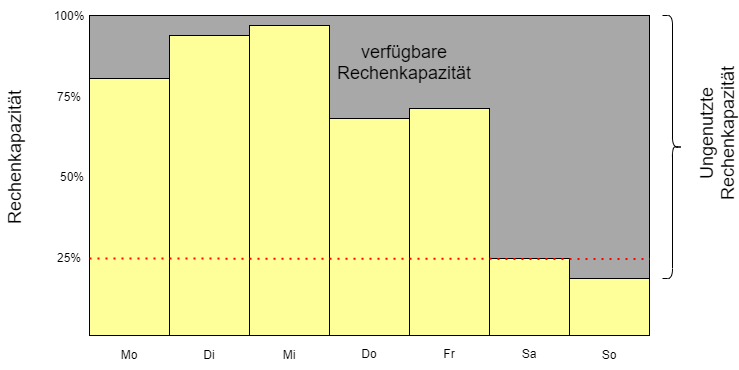
\includegraphics[scale=0.5]{sources/AutoCap Unused Capacity}
    \caption[Ungenutzte Rechenkapazität ohne automatische Skalierung]{}
    \label{fig:AutoSca_Unused_Capacity} Ungenutzte Rechenkapazität ohne automatische Skalierung. \\
    Quelle: Eigene Darstellung. 
    %\footnote{\cite{AMZ01}}
  \end{figure}

%Zu erklären: cooldown period and scaling policy.
%Macht die Nutzung von Spor-Instanzen so einfach wie nie zuvor ?

\subsubsection{Zeitgesteuerte Skalierung}
%WE für Dev und Beta
\textbf{Nicht produktive Umgebungen??}

In einem On-Premise-System macht es möglicherweise keinen Unterschied bei den Kosten, wenn die Instanzen aktiv bleiben. 
Im Gegensatz dazu ist es bei On-Demand-Zahlungsmodelle sinnvoll Zeiträume zu definieren, in denen die Instanzen abgeschaltet werden sollen.

Bei Systemen, die nur tagsüber und unter der Woche in Betrieb sein müssen, kann dies eine Einsparung von zu 67\% bedeuten.  Wenn zum Beispiel Test- und Beta-Umgebungen von Montag bis Freitag von 7 bis 20 Uhr laufen.
[DAS WÜRDE IN EUROS GESPART WERDEN: BEISPIEL Stundensatz x Stunden]
% Automatisiere das Hoch- und Herunterfahren von Instanzen
% https://www.linkedin.com/learning/monitoring-aws-with-cloudwatch/autoscaling-using-alarms?autoAdvance=true&autoSkip=true&autoplay=true&resume=false&u=79182202

% Grund: weil i.d.R., kein Entwickler 24/7 arbeitet.
% Wie?: mit Tagging, Lambda oder mit Auto Scaling Groups.
%Wann ist es sinnvoll Systeme runterzufahren 
%HIER LESEN {\cite{CCB}, Seite 153}

%Weihnachten und BackFriday
\textbf{Produktive Umgebungen??}
Wenn der Zeitpunkt einer hohen Nachfrage bekannt ist, kann eine Erhöhung der Rechnerkapazität geplant werden, um Überlastungen zu vermeiden.

Beispiele für solche Zeiträume sind Weihnachten, Cyber-Monday und Black Friday. 
[STATISTIK?]

\subsubsection{Dynamische automatische Skalierung / Dynamisches Auto Scaling}
%Intro mit Beispiel
Es kann jedoch zu schnelle und kontinuierliche Änderungen im Verhalten von Applikationen geben, bei denen es sinnvoller ist, Metriken zur Anpassung der Skalierung der Rechenkapazität festzulegen.

Beispiele für eine veränderte Nutzung von Applikationen finden sich bei Tinder und OkCupid, zwei der größten Dating-Applikationen in den vereinigten staaten. Die \autoref{fig:Use_by_hour_netflix_OkCupid_tinder} zeigt die Nutzungsspitzen bei den genannten Applikationen. Dieses wechselnde Verhalten wirkt sich unmittelbar auf die zu verschiedenen Tageszeiten benötigte Rechenkapazität aus und macht eine dynamische Skalierung der Rechenkapazität erforderlich, wenn das Ziel darin besteht, die Verschwendung von Ressourcen zu vermeiden oder zu verringern. 
\begin{figure}[h!]
  \centering
  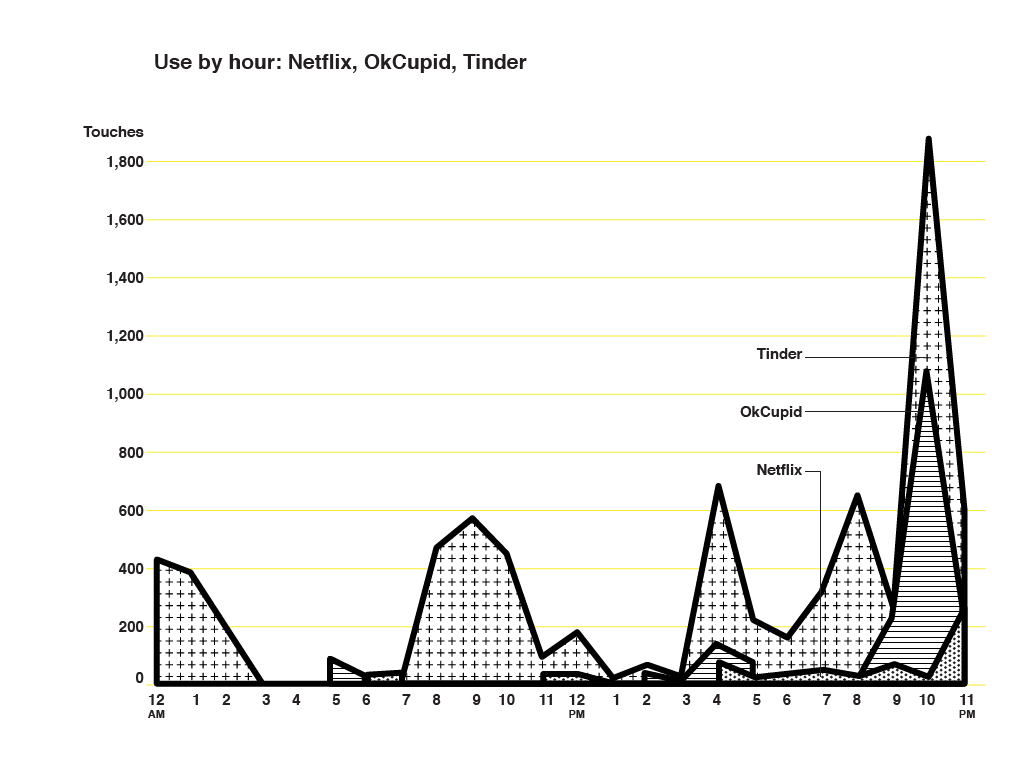
\includegraphics[scale=0.33]{sources/Use_by_hour_netflix_OkCupid_tinder}
  \caption[Nutzung von Tinder, OkCupid und Netflix pro Stunde]{}\label{fig:Use_by_hour_netflix_OkCupid_tinder} Nutzung von Tinder, OkCupid und Netflix pro Stunde.  
  %Quelle: Eigene Darstellung. 
  {\cite{SCOUT1}}
  \\Mit Touches sind die Anzahl der Klicks, Swipes oder einfachen Interaktionen mit der Applikation gemeint.
\end{figure}

Weitere Beispiele für solche Zeitpunkte sind das Feierabend, Mittagspause und beim Abendessen, wenn es um Applikationen für Unterhaltung und Online-Shopping geht.
\\
%HIER erkläre ich wie genau AutoScaling funktioniert und was dafür nötig ist (Metriken)
Die für die automatische Skalierung erforderlichen Metriken wurden bereits im Kapitel Überwachungswerkzeuge erwähnt. Eine der Metriken, die von Optimierungsexperten [PASST?]benutzt wird, ist die gesamte CPU-Auslastung. 
Um die CPU-Auslastung als Metrik zu verwenden, werden mindestens zwei Schwellenwerte definiert. Eine für die Erhöhung von Rechenkapazität (Scale-Out) und eine für das Verringern von Rechenkapazität (Scale-In).


\subsubsection{Voraussagende Skalierung / Predective Scaling ??}
Voraussagende Skalierung oder Predictive Scaling auf Englisch, nutzt maschinelles Lernen, um den Kapazitätsbedarf auf der Grundlage historischer Daten von CloudWatch vorherzusagen. Mit Hilfe der Predictive Scaling kann es die Kapazität vor der erwarteten Auslastung bereitstellen, im Gegensatz zur dynamischen Skalierung, die reaktiv ist. 
Für Instanzen, die viel Zeit für die Initialisierung benötigen kann die Zeit zwischen dem Beginn des Nachfrageanstiegs und der Initialisierung der Instanz vermieden oder verkürzt werden.
[DIAGRAMM]
Anders als Zeitgesteuerte Skalierung ist es nicht notwendig, die Verhaltensmuster der Anwendungen zu analysieren.
[SOLLTE DAS ZITIERT WERDEN?]
%https://docs.aws.amazon.com/autoscaling/ec2/userguide/as-dg.pdf#ec2-auto-scaling-predictive-scaling

\subsubsection{ Manual Scaling REVIEWEN}
Wenn aufgrund von Bedingungen, die in der Konfiguration unserer Auto-Scaling-Gruppe nicht berücksichtigt sind, mehr Rechenkapazität benötigt wird, ist es möglich, die Rechenkapazität manuell zu ändern. Die minimale, die maximale oder die gewünschte Kapazität der Auto-Scaling-Gruppe kann verändert werden,, ohne dass aktive Instanzen unterbrochen werden müssen.








\subsection{S3 Optimierung}

\subsubsection{Richtige Speicherklassen wählen}
Um die Speicherkosten zu optimieren, ist es daher notwendig, die richtige Speicherklassen für die jeweilige Applikation wählen. Um die richtige Wahl zu treffen, müssen die Anforderungen der Applikation verstanden werden. Klinische Patientendaten und eine Instagram-Story unterscheiden sich in der Zugriffshäufigkeit auf diese Daten und in der Länge der Aufbewahrungszeit[PASSENDES WORT?].

Amazon bietet verschiedene Speicherklassen an, die sich im Preis und in der Häufigkeit des Zugriffs auf die Objekte unterscheiden. Objekte sind in Behältern enthalten, die Buckets genannt werden.
[ABB Speicherklasse ->Eigenschaften der Anwendung?]
LIFE-CYCLE-POLICIES
%WICHTIG IST DIE GRÖSSE MEINE DATEIEN UND DIE ANZAHL.
%weil SO WERDEN DIE PREISE FÜR VERSCHIEBUNG BERECHNET.
%(Object size distribution )

\subsubsection{Intelligent Auto Tiering}
Intelligent Auto Tiering verschiebt Daten auf der Grundlage von Zugriffsmustern. Diese Speicherklasse ist ideal für Daten mit wechselnden oder unbekannten Zugriffsmustern. 
Wie die Senior Product Manager für S3 Ruhi Dang erklärt, einige Unternehmen haben weder die Zeit noch die finanziellen Möglichkeiten, eine Person einzustellen, die ihre Daten sortiert und in die richtige Art von Speicher einordnet. Intelligent Auto Tiering ist eine attraktative Lösung für Firmen, die jährlich weniger als \$100,000 für Speicher ausgeben \footnote{\cite{AMZ16}, Minute: 21:12}.
%Ach von Jessie Felix gesagt https://www.youtube.com/watch?v=IOT41L_adSw

\begin{figure}[h!]
  \centering
  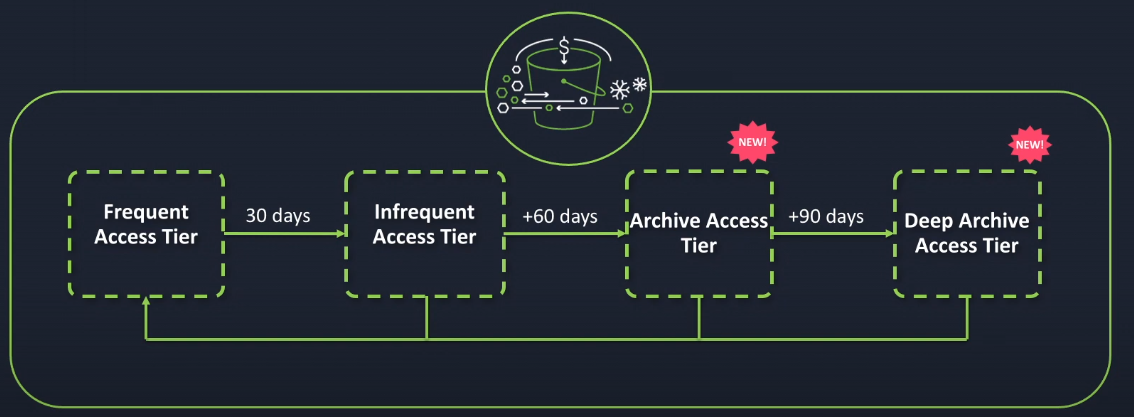
\includegraphics[scale=0.5]{sources/S3_IntLifeCycle}
  \caption[Funktionsweise von Intelligent-Tiering]{}\label{fig:S3_IntLifeCycle} Funktionsweise von Intelligent-Tiering\\
  MACH DIR EINE ÄHLICHE ABER DEINES
  %Quelle: Eigene Darstellung. 
  %{\cite{SCOUT1}}
\end{figure}


IDEAL FUR DATA LAKES,DATA SCIENCE /MACHINES LEARNING

















\begin{comment}
\subsubsection{Automatisierung mit Lambda Funktionen}
Grund: einmal programmiert, funktioniert es für immer.
\\(To-Do:) Möglichkeiten untersuchen, bewerten und die passende Auswählen.

%Limitierung 
%Quotas setzen? erweitern oder reduzieren / benachrichtigen aber auch eine Aktion durchführen 

%Lambda

AWS Lambda is a compute service. You can use it to run code without provisioning or managing servers. Lambda runs your code on a high-availability compute infrastructure. It operates and maintains all of the compute resources, including server and operating system maintenance, capacity provisioning and automatic scaling, code monitoring, and logging. With Lambda, you can run code for almost any type of application or backend service. 

Some benefits of using Lambda include the following:

You can run code without provisioning or maintaining servers.
It initiates functions for you in response to events.
It scales automatically.
It provides built-in code monitoring and logging via Amazon CloudWatch.
\end{comment}

%Data Pipeline

%Economic Performance?
%QUEUES

%NEVER forget your availability requirements, trying to optimize, first availability THEN cost...
%Do not use your DB for saving BLOB

%\subsection{VERKAUFE DEINE Ungenutzte Kapazität in RI Marketplace}

%Kombination
%https://spot.io/blog/effective-utilization-of-aws-savings-plans-and-ec2-spot-instances/#a1
%https://www.youtube.com/watch?v=X_7pnzPlESs

 